\section{Zielsetzung}
\label{sec:Zielsetzung}

Ziel des Versuches ist es das Anregungs- und Dämpfungsverhalten eines LRC-Schwingkreises
bei Wechselstrom verschiedener Frequenzen zu beschreiben.


\section{Theorie}
\label{sec:Theorie}

\subsection{Dämpfung des Stroms in einem Schwingkreis}
Zunächst wird der folgende Schwingkreis betrachtet, welcher durch einen
kurzen Strompuls in Gang gesetzt wird und danach abklingt.
\begin{figure}[H]
  \centering
  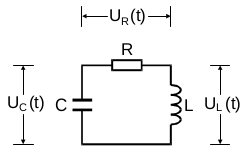
\includegraphics{content/images/V354.png}
  \caption{Gedämpfter L-R-C-Schwingkreis\cite{anleitung}.}
  \label{fig:schwingkreis}
\end{figure}
Für den Stromkreis in Abbildung \ref{fig:schwingkreis} gilt die
DGL:
\begin{equation}
  U_C(t)+U_R(t)+U_L(t)=0
\end{equation}
Diese lässt sich umformen zu
\begin{equation}
  L\frac{\symup{d}\, I}{\symup{d}\, t} +RI +\frac{Q}{C}=0
\end{equation}
mit
\begin{equation}
  I = \frac{\symup{d}\, Q}{\symup{d}\, t}
\end{equation}
Für den beschriebenen Strompuls kann die Lösung der DGL mathematisch durch die Überlagerung einer
einhüllenden Funktion und einer sinus/cosinus Funktion dargestellt werden.
\begin{figure}[H]
  \centering
  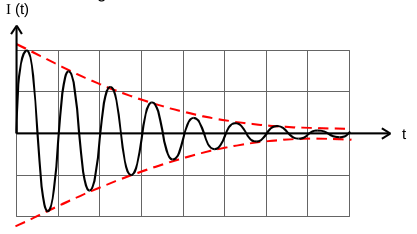
\includegraphics{content/images/dia.png}
  \caption{Dämpfungskurve des Stroms\cite{anleitung}.}
  \label{fig:daempfung}
\end{figure}
\begin{align}
  \symbf{I} &= I_0 e^{-2\pi\mu t}
  \cdot\text{cos}\left(2\pi\nu t+\eta\right)\\
  \symbf{I}_\text{einhüllend} &= I_0 e^{-2\pi\mu t}
  \label{eqn:einhuellend}
\end{align}
mit der Definition
\begin{align}
  2\pi\mu&\coloneq\frac{R}{2L}\\
  \intertext{und}
  2\pi\mu&\coloneq\sqrt{\frac{1}{LC}-\frac{R^2}{4L^2}}
\end{align}
sowie der Phase $\eta$.
Die Abklingdauer wird nach
\begin{equation}
  T_{\text{ex}}\coloneq\frac{1}{2\pi\mu} = \frac{2L}{R}
  \label{tex}
\end{equation}
und der Dämpfungswiderstand nach
\begin{equation}
  R_{\text{eff}}= 4\pi\mu L
  \label{reff}
\end{equation}
berechnet.

\subsection{Grenzwiderstand für den aperiodischen Grenzfall}
\begin{figure}[H]
  \centering
  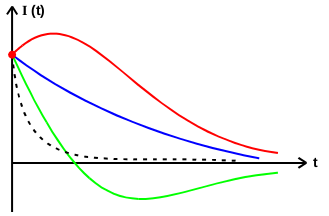
\includegraphics{content/images/dia2.png}
  \caption{Dämpfungskurve des Stroms\cite{anleitung}.}
  \label{fig:aperiodisch}
\end{figure}
Nach der Bestimmung des Dämpfungsverhaltens eines Schwingkreises
wird nun der Widerstand $R_\text{ap}$ berechnet für welchen der
Strom im Schwingkreis am schnellsten gegen null läuft. Dieses
Phänomen wird aperiodischer Grenzfall genannt und wird durch
die gestrichelte Linie in Abbildung \ref{fig:aperiodisch}
dargestellt. Es tritt auf wenn $2\pi\mu=2\pi\eta$ gilt. Ist $2\pi\mu\geq 2\pi\eta$, so wirkt die Gegeninduktion der
Spule verlangsamend und es kommt zum Kriechfall wie beim blauen Graph in Abbildung \ref{fig:aperiodisch}, ist
$2\pi\mu$ etwas kleiner als $2\pi\eta$
ergibt sich ein Anschwingen wie beim grünen Graphen. Ein weiterer möglicher
Verlauf ist das Überschwingen, welches durch den roten Graphen abbgebildet ist.
Mathematisch lässt sich dies über die Periodendauer T des
Schwingkreises bestimmen.
\begin{equation}
  T = \frac{1}{\eta} = \frac{2\pi}{\sqrt{1/LC-R^2/4L^2}}
\end{equation}
Der Grenzfall tritt für $T\to\infty$ auf:
\begin{equation}
  \implies \frac{1}{LC}=\frac{R_\text{ap}^2}{4L^2}
\end{equation}
\begin{equation}
  \iff R_\text{ap} =\sqrt{\frac{4L}{C}}
  \label{eqn:R11}
\end{equation}

\subsection{Frequenzabhängigkeit der Kondensatorspannung}
\begin{figure}[H]
  \centering
  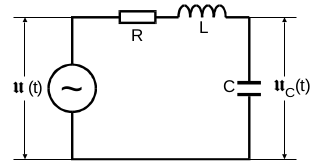
\includegraphics{content/images/kreis2.png}
  \caption{angeregter Schwingkreis\cite{anleitung}.}
  \label{fig:kreis2}
\end{figure}
Für die folgenden Versuchsteile wird ein erzwungener Schwingkreis
wie in Abbildung \ref{fig:kreis2} verwendet. Die DGL lautet nun:
\begin{equation}
  U_C(t)+U_R(t)+U_L(t)=U_0e^{i\omega t}
\end{equation}
Dies lässt sich umformen zu:
\begin{equation}
  L\frac{\symup{d}\, I}{\symup{d}\, t} +RI +\frac{Q}{C}=U_0e^{i\omega t}
  \label{eqn:kreis3}
\end{equation}
Der Ansatz für die DGL lautet:
\begin{equation}
  U_\symup{C}(\omega , t)= U(\omega)e^{i\omega t}
\end{equation}
und es ergibt sich für $U(\omega)$:
\begin{equation}
  -LC\omega^2U(\omega)+i\omega RCU(\omega)+U(\omega)=U_0
  \label{eqn:lsg}
\end{equation}
Die Eigenfrequenz $\omega_0$ dieses Kreises beträgt:
\begin{equation}
  \omega_0=\frac{1}{\sqrt{LC}}
  \label{eqn:eigen}
\end{equation}
Zunächst wird die Güte $q$ durch die Abhängigkeit
der Kondensatorspannung $U_C$ von der Kreisfrequenz $\omega$ berechnet:
\begin{equation}
  q_\text{exp}=\frac{U_c}{U_\text{erreger}}
  \label{eqn:qexp}
\end{equation}
Hierbei ist der Umrechnungsfaktor der gemessenen Frequenz $\nu$ zur Kreisfrequenz $\omega$
zu beachten:
\begin{equation}
  \omega = 2\pi\nu
  \label{c1}
\end{equation}
Diese wird verglichen mit der theoretischen Güteziffer welche sich durch die physikalischen
Eigenschaften des Schwingkreises, sprich $L$, $R$ und $C$, berechnen lässt:
\begin{equation}
  q_\text{theo}=\frac{1}{R}\sqrt{\frac{L}{C}}
    \label{eqn:qtheo}
\end{equation}
Trägt man $U_C$ gegen $\omega$ auf erhält man eine Glockenkurve deren Breite errechnet wird durch:
\begin{equation}
  \omega_+-\omega_-=\frac{R}{L}
  \label{eqn:breite}
\end{equation}

\subsection{Frequenzabhängigkeit der Phase}
Des weiteren lässt sich eine Phase $\phi$ zwischen der Erregerspannung
$U_\text{erreger}$ und der Kondensatorspannung $U_\text{kondensator}$  feststellen und über
die Lösung \eqref{eqn:lsg} der DGL \eqref{eqn:kreis3} unter Berücksichtigung der komplexen Impendanz $Z$ berechnen nach:
\begin{equation}
  \phi = \text{arctan}\left(\frac{-\omega RC}{1-LC\omega^2}\right)
  \label{eqn:phase}
\end{equation}
Daraus ergeben sich $\omega_\text1$ und $\omega_\text2$ nach
\begin{equation}
  \omega_{1/2} = \pm \frac{R}{2L} + \sqrt{\frac{R^{2}}{4L^{2}} + \frac{1}{LC}}
  \label{o12}
\end{equation}
für $\phi = \frac{\pi}{4}\,\text{und}\, \frac{3\,\pi}{4}$ und $\omega_\text{res}$ nach
\begin{equation}
  \omega_\text{res}=\sqrt{\frac{1}{LC}-\frac{R^2}{2L^2}}
  \label{eqn:ores}
\end{equation}
für $\phi = \frac{\pi}{2}$.
Die Phase wird durch eine Zeitdifferenz $\symup{d}t$ der Nulldurchgänge bei einer Frequenz $\nu$
berechnet:
\begin{equation}
  \phi = \omega \symup{d}t = 2\pi\nu \symup{d}t
\end{equation}
